\chapter{Généralités sur les systèmes oscillants}

\textit{Des battements du cœur aux oscillations d'un pendule, en passant par les courants alternatifs, les phénomènes oscillatoires sont omniprésents dans la nature et la technologie. Ce chapitre pose les bases de l'étude des systèmes oscillants : grandeurs caractéristiques, représentation mathématique et graphique, classification des oscillations, et introduction au phénomène de résonance.}

\section{Phénomènes périodiques et grandeurs associées}

\subsection{Définition d'un phénomène périodique}

\begin{definition}[Phénomène périodique]
Un phénomène est dit \textbf{périodique} lorsqu'il se reproduit identique à lui-même à intervalles de temps égaux, appelés \textbf{périodes}.
\end{definition}

\begin{exemple}
\begin{itemize}
\item Le mouvement d'un pendule simple (oscillations).
\item La tension du secteur électrique (\SI{50}{\hertz} en Europe, \SI{60}{\hertz} aux États-Unis).
\item Les battements du cœur humain (environ \SI{1.2}{\hertz} au repos).
\end{itemize}
\end{exemple}

\subsection{Période, fréquence et pulsation}

\begin{definition}[Période $T$]
La \textbf{période} $T$ est la plus petite durée au bout de laquelle le phénomène se reproduit identique à lui-même. Elle s'exprime en \si{\second}.
\end{definition}

\begin{definition}[Fréquence $f$]
La \textbf{fréquence} $f$ est le nombre de répétitions du phénomène par unité de temps. Elle s'exprime en \si{\hertz} (\si{\per\second}).
\[
f = \frac{1}{T}
\]
\end{definition}

\begin{definition}[Pulsation $\omega$]
La \textbf{pulsation} $\omega$ (ou fréquence angulaire) est liée à la fréquence et à la période par :
\[
\omega = 2\pi f = \frac{2\pi}{T}
\]
Elle s'exprime en \si{\radian\per\second}.
\end{definition}

\begin{aretenir}
Pour tout phénomène périodique :
\[
\boxed{T = \frac{1}{f} = \frac{2\pi}{\omega}} \qquad \boxed{f = \frac{1}{T} = \frac{\omega}{2\pi}} \qquad \boxed{\omega = 2\pi f = \frac{2\pi}{T}}
\]
\end{aretenir}

\begin{exemple}
Un diapason émet un son de fréquence \SI{440}{\hertz}. Sa période est :
\[
T = \frac{1}{f} = \frac{1}{440} \approx \SI{2.27e-3}{\second} = \SI{2.27}{\milli\second}
\]
Sa pulsation est :
\[
\omega = 2\pi f = 2\pi \times 440 \approx \SI{2765}{\radian\per\second}
\]
\end{exemple}

\section{Grandeurs sinusoïdales}

\subsection{Définition et représentation mathématique}

\begin{definition}[Grandeur sinusoïdale]
Une grandeur physique $y(t)$ est dite \textbf{sinusoïdale} (ou harmonique) si elle varie au cours du temps selon une fonction sinus ou cosinus :
\[
y(t) = Y_m \cos(\omega t + \varphi) \quad \text{ou} \quad y(t) = Y_m \sin(\omega t + \varphi)
\]
où :
\begin{itemize}
\item $Y_m$ est l'\textbf{amplitude} (valeur maximale) de la grandeur ;
\item $\omega$ est la \textbf{pulsation} (en \si{\radian\per\second}) ;
\item $\varphi$ est la \textbf{phase à l'origine} (en \si{\radian}) ;
\item $(\omega t + \varphi)$ est la \textbf{phase instantanée}.
\end{itemize}
\end{definition}

\begin{remarque}
Les fonctions sinus et cosinus sont reliées par : $\sin\theta = \cos(\theta - \pi/2)$. On peut donc toujours exprimer une grandeur sinusoïdale sous forme d'un cosinus.
\end{remarque}

\subsection{Amplitude, valeur crête et valeur efficace}

\begin{definition}[Amplitude et valeur efficace]
Pour une grandeur sinusoïdale $y(t) = Y_m \cos(\omega t + \varphi)$ :
\begin{itemize}
\item $Y_m$ est l'\textbf{amplitude} (ou valeur crête) ;
\item La \textbf{valeur efficace} $Y_{\text{eff}}$ est définie par :
\[
Y_{\text{eff}} = \frac{Y_m}{\sqrt{2}}
\]
\end{itemize}
\end{definition}

\begin{exemple}
La tension du secteur en France est $U_{\text{eff}} = \SI{230}{\volt}$. Son amplitude est :
\[
U_m = U_{\text{eff}} \sqrt{2} \approx 230 \times 1.414 \approx \SI{325}{\volt}
\]
\end{exemple}

\subsection{Déphasage entre deux grandeurs sinusoïdales}

\begin{definition}[Déphasage]
Soient deux grandeurs sinusoïdales de même pulsation :
\[
y_1(t) = Y_{1m} \cos(\omega t + \varphi_1) \quad \text{et} \quad y_2(t) = Y_{2m} \cos(\omega t + \varphi_2)
\]
Le \textbf{déphasage} de $y_2$ par rapport à $y_1$ est :
\[
\Delta\varphi = \varphi_2 - \varphi_1
\]
\end{definition}

\begin{propriete}[Interprétation du déphasage]
\begin{itemize}
\item Si $\Delta\varphi > 0$ : $y_2$ est \textbf{en avance} sur $y_1$.
\item Si $\Delta\varphi < 0$ : $y_2$ est \textbf{en retard} sur $y_1$.
\item Si $\Delta\varphi = 0$ : les grandeurs sont \textbf{en phase}.
\item Si $\Delta\varphi = \pm\pi$ : les grandeurs sont \textbf{en opposition de phase}.
\item Si $\Delta\varphi = \pm\pi/2$ : les grandeurs sont \textbf{en quadrature}.
\end{itemize}
\end{propriete}

\begin{illus}
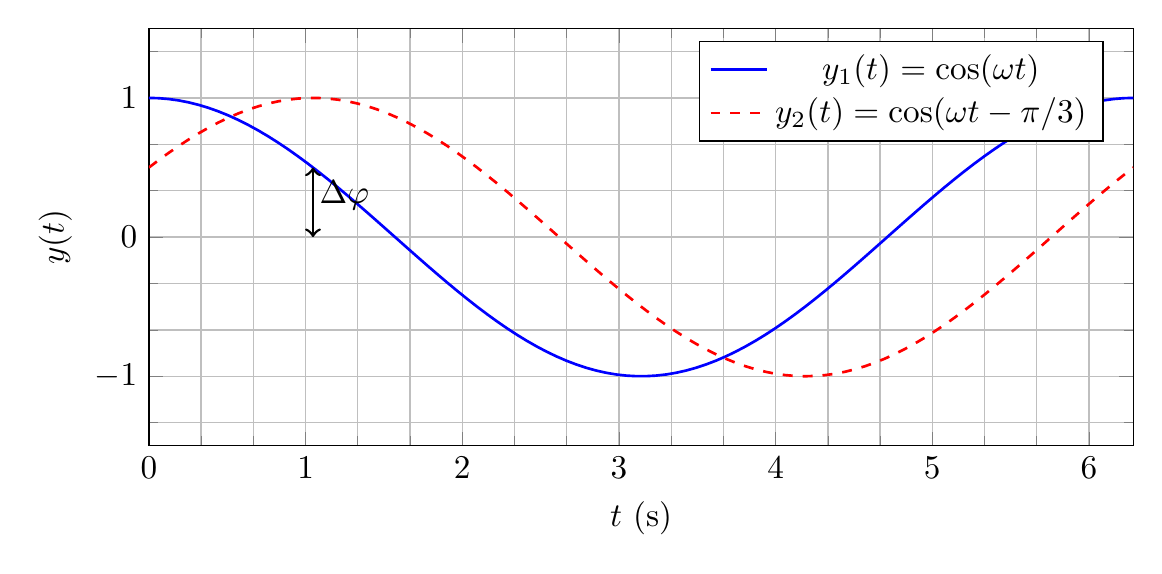
\begin{tikzpicture}[scale=1.2]
\begin{axis}[
    width=12cm, height=6cm,
    xlabel={$t$ (s)}, ylabel={$y(t)$},
    xmin=0, xmax=2*pi,
    ymin=-1.5, ymax=1.5,
    domain=0:2*pi,
    samples=100,
    legend pos=north east,
    grid=both,
    minor tick num=2,
    ]
    \addplot[thick, blue] {cos(deg(x))};
    \addlegendentry{$y_1(t) = \cos(\omega t)$}
    \addplot[thick, red, dashed] {cos(deg(x - pi/3))};
    \addlegendentry{$y_2(t) = \cos(\omega t - \pi/3)$}
    \draw[<->, thick] (axis cs:{pi/3},0) -- (axis cs:{pi/3},{cos(deg(pi/3))});
    \node at (axis cs:{pi/3+0.2},0.3) {$\Delta\varphi$};
\end{axis}
\end{tikzpicture}
\fig{Figure 5.1 — Représentation temporelle de deux signaux sinusoïdaux déphasés de $\pi/3$.}
\end{illus}

\section{Représentation de Fresnel}

\subsection{Principe de la représentation}

\begin{definition}[Vecteur de Fresnel]
À toute grandeur sinusoïdale $y(t) = Y_m \cos(\omega t + \varphi)$, on associe un \textbf{vecteur tournant} (ou vecteur de Fresnel) $\vect{Y}$ tel que :
\begin{itemize}
\item Sa longueur est égale à l'amplitude $Y_m$ ;
\item Il fait un angle $\varphi$ avec l'axe de référence à $t=0$ ;
\item Il tourne à la vitesse angulaire $\omega$ dans le sens trigonométrique.
\end{itemize}
La projection de $\vect{Y}$ sur l'axe horizontal donne $y(t)$.
\end{definition}

\begin{illus}
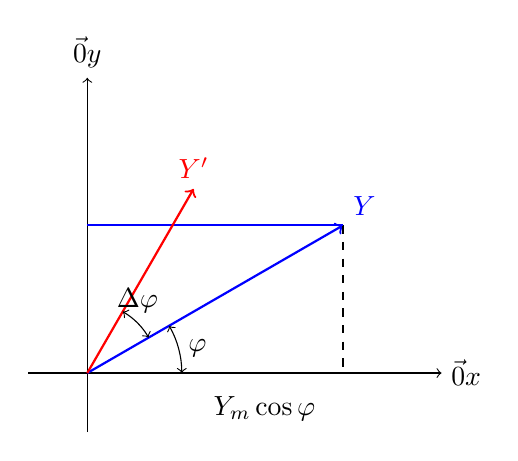
\begin{tikzpicture}[scale=1.5]
\draw[->] (-0.5,0) -- (3,0) node[right] {$\vec{0}x$};
\draw[->] (0,-0.5) -- (0,2.5) node[above] {$\vec{0}y$};
\draw[->, thick, blue] (0,0) -- (30:2.5) node[above right] {$\vect{Y}$};
\draw[dashed] (30:2.5) -- (30:2.5 |- 0,0);
\draw[<->] (0:0.8) arc (0:30:0.8) node[midway, right] {$\varphi$};
\draw[thick, blue] (30:2.5) -- (30:2.5 -| 0,0);
\node at (1.5,-0.3) {$Y_m \cos\varphi$};
\draw[->, thick, red] (0,0) -- (60:1.8) node[above] {$\vect{Y}'$};
\draw[<->] (30:0.6) arc (30:60:0.6) node[midway, above] {$\Delta\varphi$};
\end{tikzpicture}
\fig{Figure 5.2 — Diagramme de Fresnel : deux vecteurs représentant deux grandeurs sinusoïdales déphasées.}
\end{illus}

\subsection{Addition de grandeurs sinusoïdales}

\begin{propriete}[Somme de deux grandeurs sinusoïdales de même pulsation]
La somme de deux grandeurs sinusoïdales de même pulsation est une grandeur sinusoïdale de même pulsation. Son amplitude et sa phase se déterminent graphiquement par la somme vectorielle des vecteurs de Fresnel associés.
\end{propriete}

\begin{exemple}
Soient $y_1(t) = 3\cos(\omega t)$ et $y_2(t) = 4\cos(\omega t + \pi/2)$. Le vecteur résultant a pour amplitude :
\[
Y_m = \sqrt{3^2 + 4^2} = 5
\]
et pour phase :
\[
\varphi = \arctan\left(\frac{4}{3}\right) \approx \SI{0.927}{\radian}
\]
Donc $y(t) = 5\cos(\omega t + 0.927)$.
\end{exemple}

\section{Classification des oscillations}

\subsection{Oscillations libres et forcées}

\begin{definition}[Oscillations libres]
Un système effectue des \textbf{oscillations libres} lorsqu'il oscille sous l'effet de sa seule énergie initiale, sans entretien extérieur.
\end{definition}

\begin{definition}[Oscillations forcées]
Un système effectue des \textbf{oscillations forcées} lorsqu'il est soumis à une excitation extérieure périodique (force excitatrice). Il oscille alors à la fréquence de l'excitation.
\end{definition}

\subsection{Oscillations amorties et non amorties}

\begin{definition}[Oscillations amorties]
Des oscillations sont dites \textbf{amorties} lorsque leur amplitude diminue au cours du temps à cause de frottements ou de pertes d'énergie.
\end{definition}

\begin{definition}[Oscillations non amorties]
Des oscillations sont dites \textbf{non amorties} (ou entretenues) lorsque leur amplitude reste constante, l'énergie perdue étant compensée par un apport extérieur.
\end{definition}

\begin{illus}
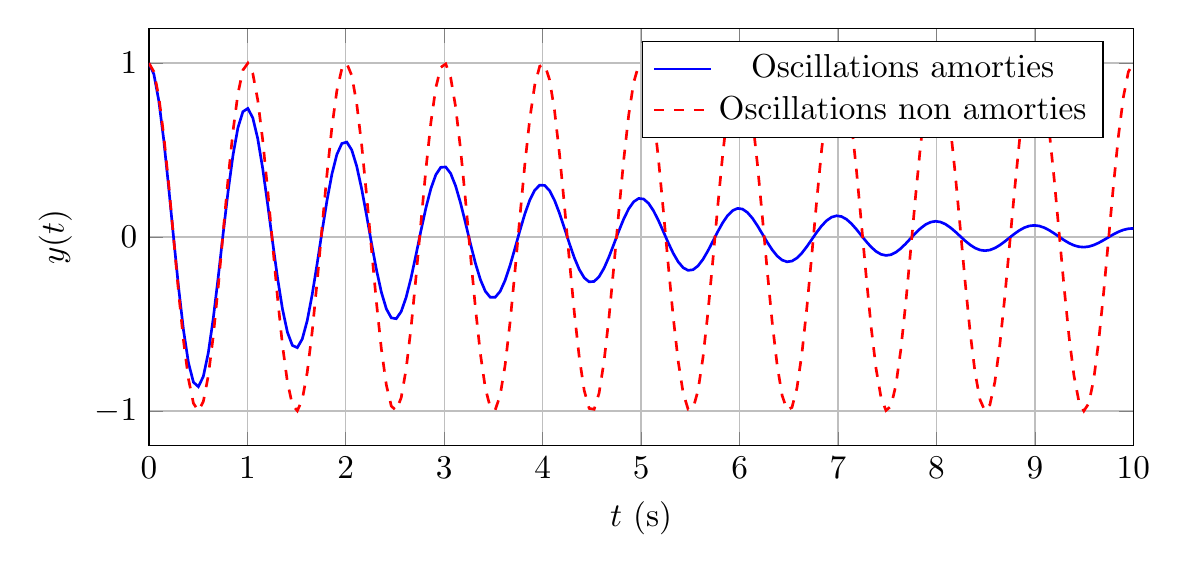
\begin{tikzpicture}[scale=1.2]
\begin{axis}[
    width=12cm, height=6cm,
    xlabel={$t$ (s)}, ylabel={$y(t)$},
    xmin=0, xmax=10,
    ymin=-1.2, ymax=1.2,
    domain=0:10,
    samples=200,
    legend pos=north east,
    grid=both,
    ]
    \addplot[thick, blue] {exp(-0.3*x)*cos(deg(2*pi*x))};
    \addlegendentry{Oscillations amorties}
    \addplot[thick, red, dashed] {cos(deg(2*pi*x))};
    \addlegendentry{Oscillations non amorties}
\end{axis}
\end{tikzpicture}
\fig{Figure 5.3 — Comparaison entre oscillations amorties et non amorties.}
\end{illus}

\section{Introduction à la résonance}

\begin{definition}[Résonance]
La \textbf{résonance} est le phénomène par lequel un système oscillant forcé présente une amplitude maximale lorsque la fréquence de l'excitation est égale à sa fréquence propre.
\end{definition}

\begin{propriete}[Caractéristiques de la résonance]
\begin{itemize}
\item À la résonance, l'amplitude des oscillations est maximale.
\item La fréquence de résonance est proche de la fréquence propre du système.
\item Plus l'amortissement est faible, plus l'amplitude à la résonance est grande et plus la résonance est aiguë.
\end{itemize}
\end{propriete}

\begin{experience}[Observation de la résonance]
\begin{itemize}
\item \textbf{Matériel} : pendule élastique (masse-ressort), excitateur à fréquence variable.
\item \textbf{Manipulation} : on fait varier la fréquence de l'excitateur et on mesure l'amplitude des oscillations du pendule.
\item \textbf{Observation} : l'amplitude est maximale lorsque la fréquence de l'excitateur est égale à la fréquence propre du pendule.
\end{itemize}
\end{experience}

\begin{remarque}
La résonance peut être bénéfique (récepteur radio accordé sur une fréquence) ou destructive (pont qui s'effondre sous l'effet du vent).
\end{remarque}

\section{L'essentiel à retenir}

\begin{synthese}
\subsection*{Grandeurs caractéristiques}
\begin{itemize}
\item \textbf{Période $T$} : durée d'un cycle complet (en \si{\second}).
\item \textbf{Fréquence $f$} : nombre de cycles par seconde (en \si{\hertz}) : $f = 1/T$.
\item \textbf{Pulsation $\omega$} : $ \omega = 2\pi f = 2\pi/T$ (en \si{\radian\per\second}).
\end{itemize}

\subsection*{Grandeur sinusoïdale}
\[
y(t) = Y_m \cos(\omega t + \varphi)
\]
\begin{itemize}
\item $Y_m$ : amplitude (valeur maximale).
\item $Y_{\text{eff}} = Y_m/\sqrt{2}$ : valeur efficace.
\item $\varphi$ : phase à l'origine.
\item $\Delta\varphi = \varphi_2 - \varphi_1$ : déphasage entre deux grandeurs.
\end{itemize}

\subsection*{Représentation de Fresnel}
\begin{itemize}
\item Vecteur de longueur $Y_m$ faisant un angle $\varphi$ avec l'axe de référence.
\item La somme de deux grandeurs sinusoïdales de même pulsation se fait par addition vectorielle.
\end{itemize}

\subsection*{Types d'oscillations}
\begin{itemize}
\item \textbf{Libres} : sans entretien extérieur.
\item \textbf{Forcées} : sous l'effet d'une excitation périodique.
\item \textbf{Amorties} : amplitude décroissante (frottements).
\item \textbf{Non amorties} : amplitude constante (apport d'énergie).
\end{itemize}

\subsection*{Résonance}
\begin{itemize}
\item Amplitude maximale quand $f_{\text{excitatrice}} = f_{\text{propre}}$.
\item Plus l'amortissement est faible, plus la résonance est aiguë.
\end{itemize}

\subsection*{Pièges à éviter}
\begin{itemize}
\item Ne pas confondre période et fréquence (inverses l'une de l'autre).
\item Ne pas oublier le facteur $2\pi$ dans le lien entre pulsation et fréquence.
\item Le déphasage se mesure en radians, pas en degrés (sauf indication contraire).
\item La valeur efficace est toujours inférieure à l'amplitude.
\end{itemize}
\end{synthese}

\section{Méthodes \& savoir-faire}

\methode{Déterminer période, fréquence et pulsation à partir d'un graphique}
Pour déterminer ces grandeurs à partir d'une courbe $y(t)$ :
\begin{enumerate}
\item Mesurer la durée $T$ entre deux maxima (ou deux passages à zéro dans le même sens).
\item Calculer $f = 1/T$ et $\omega = 2\pi f$.
\end{enumerate}

\begin{exemple}
Sur un oscillogramme, on mesure $T = \SI{20}{\milli\second}$. Alors :
\[
f = \frac{1}{20\times 10^{-3}} = \SI{50}{\hertz}, \quad \omega = 2\pi \times 50 = \SI{314}{\radian\per\second}
\]
\end{exemple}

\methode{Lire un déphasage sur un oscillogramme}
Pour deux signaux visualisés simultanément :
\begin{enumerate}
\item Mesurer le décalage temporel $\Delta t$ entre deux passages à zéro dans le même sens.
\item Calculer le déphasage : $\Delta\varphi = 2\pi \frac{\Delta t}{T}$.
\end{enumerate}

\begin{exemple}
Deux signaux de période $T = \SI{10}{\milli\second}$ présentent un décalage $\Delta t = \SI{2.5}{\milli\second}$.
\[
\Delta\varphi = 2\pi \times \frac{2.5}{10} = \frac{\pi}{2} \ \si{\radian}
\]
Le second signal est en quadrature retard par rapport au premier.
\end{exemple}

\methode{Construire un diagramme de Fresnel}
Pour représenter $y(t) = Y_m \cos(\omega t + \varphi)$ :
\begin{enumerate}
\item Tracer un axe horizontal de référence.
\item À partir de l'origine, tracer un segment de longueur $Y_m$ faisant un angle $\varphi$ avec l'axe.
\item Pour additionner deux grandeurs, construire la somme vectorielle.
\end{enumerate}

\begin{exemple}
Soient $y_1(t) = 2\cos(\omega t)$ et $y_2(t) = 3\cos(\omega t + \pi/3)$. Le vecteur résultant a pour composantes :
\[
X = 2 + 3\cos(\pi/3) = 2 + 1.5 = 3.5, \quad Y = 0 + 3\sin(\pi/3) = 3 \times 0.866 = 2.598
\]
D'où $Y_m = \sqrt{3.5^2 + 2.598^2} \approx 4.36$ et $\varphi = \arctan(2.598/3.5) \approx \SI{0.64}{\radian}$.
\end{exemple}

\methode{Distinguer oscillations libres, forcées, amorties}
\begin{itemize}
\item \textbf{Libres} : pas d'excitation extérieure, le système oscille à sa fréquence propre.
\item \textbf{Forcées} : excitation extérieure périodique, fréquence imposée par l'excitateur.
\item \textbf{Amorties} : amplitude qui diminue (enveloppe exponentielle décroissante).
\end{itemize}

\begin{exemple}
Un enfant sur une balançoire qu'on pousse régulièrement : oscillations forcées. Si on arrête de pousser : oscillations libres amorties.
\end{exemple}

\section{Exercices d'application}

\rubrique{Période, fréquence, pulsation}

\exo{}\diff{1} Un pendule simple effectue 20 oscillations en \SI{40}{\second}. Calculer sa période, sa fréquence et sa pulsation.

\exo{}\diff{1} La tension du secteur au Cameroun a une fréquence de \SI{50}{\hertz}. Calculer sa période et sa pulsation.

\exo{}\diff{2} Un signal sinusoïdal a pour période $T = \SI{2.5}{\milli\second}$. Quelle est sa fréquence en \si{\hertz} ? Sa pulsation en \si{\radian\per\second} ?

\rubrique{Grandeurs sinusoïdales et déphasage}

\exo{}\diff{1} Une tension sinusoïdale a pour expression $u(t) = 12\cos(100\pi t)$. Déterminer son amplitude, sa pulsation, sa fréquence et sa période.

\exo{}\diff{2} Deux tensions sont données par $u_1(t) = 5\cos(100\pi t)$ et $u_2(t) = 5\cos(100\pi t + \pi/4)$. Calculer le déphasage de $u_2$ par rapport à $u_1$. Laquelle est en avance ?

\exo{}\diff{2} Un courant sinusoïdal a une valeur efficace de \SI{2}{\ampere} et une fréquence de \SI{60}{\hertz}. Écrire son expression temporelle sachant que sa phase à l'origine est nulle.

\rubrique{Représentation de Fresnel}

\exo{}\diff{2} Représenter sur un diagramme de Fresnel les grandeurs $y_1(t) = 3\cos(\omega t)$ et $y_2(t) = 4\cos(\omega t + \pi/2)$. En déduire graphiquement l'amplitude et la phase de la somme $y(t) = y_1(t) + y_2(t)$.

\exo{}\diff{3} Deux grandeurs sinusoïdales de même pulsation ont pour amplitudes $Y_{1m} = 5$ et $Y_{2m} = 3$, avec un déphasage de $\pi/3$. Déterminer par le calcul l'amplitude et la phase de leur somme.

\rubrique{Oscillations et résonance}

\exo{}\diff{1} Un système masse-ressort a une fréquence propre de \SI{2}{\hertz}. On l'excite à la fréquence de \SI{1.5}{\hertz}. S'agit-il d'oscillations libres ou forcées ? À quelle fréquence le système oscille-t-il ?

\exo{}\diff{2} On observe l'amplitude d'un oscillateur forcé en fonction de la fréquence d'excitation. L'amplitude maximale est obtenue pour $f = \SI{10}{\hertz}$. Que peut-on dire de la fréquence propre du système ?

\exo{}\diff{2} Un oscillateur amorti a une amplitude qui diminue de moitié tous les \SI{5}{\second}. Si l'amplitude initiale est de \SI{10}{\centi\metre}, quelle sera l'amplitude après \SI{15}{\second} ?

\section{Exercices d'entraînement}

\rubrique{Période, fréquence, pulsation}

\exo{}\diff{1} Un mouvement de rotation uniforme effectue 120 tours par minute. Calculer sa fréquence en \si{\hertz} et sa période en \si{\second}.

\exo{}\diff{2} La période d'un signal est $T = \SI{0.02}{\second}$. Calculer sa fréquence et sa pulsation.

\exo{}\diff{2} Un diapason émet un son de fréquence \SI{512}{\hertz}. Quelle est sa période ? Combien d'oscillations complètes effectue-t-il en \SI{2}{\second} ?

\exo{}\diff{3} Un signal a pour pulsation $\omega = \SI{500}{\radian\per\second}$. Calculer sa fréquence et sa période.

\rubrique{Grandeurs sinusoïdales}

\exo{}\diff{1} Une tension sinusoïdale a pour expression $u(t) = 230\sqrt{2}\cos(100\pi t)$. Quelle est sa valeur efficace ? Sa fréquence ?

\exo{}\diff{2} Un courant sinusoïdal a une amplitude de \SI{5}{\ampere} et une fréquence de \SI{50}{\hertz}. Écrire son expression si la phase à l'origine est $-\pi/6$.

\exo{}\diff{2} La valeur efficace d'une tension sinusoïdale est \SI{110}{\volt}. Quelle est son amplitude ?

\exo{}\diff{3} Deux signaux sinusoïdaux de même fréquence ont pour expressions $y_1(t) = 2\cos(200\pi t)$ et $y_2(t) = 3\cos(200\pi t + \pi/2)$. Déterminer l'expression de leur somme.

\rubrique{Déphasage}

\exo{}\diff{2} Deux tensions sont données par $u_1(t) = 10\cos(100\pi t)$ et $u_2(t) = 10\sin(100\pi t)$. Calculer le déphasage de $u_2$ par rapport à $u_1$.

\exo{}\diff{2} Sur un oscilloscope, deux signaux de période $T = \SI{1}{\milli\second}$ sont décalés de $\SI{0.125}{\milli\second}$. Quel est leur déphasage ?

\exo{}\diff{3} Trois grandeurs sinusoïdales de même pulsation ont pour phases $\varphi_1 = 0$, $\varphi_2 = \pi/3$, $\varphi_3 = 2\pi/3$. Calculer les déphasages $\varphi_{2/1}$, $\varphi_{3/2}$ et $\varphi_{3/1}$.

\rubrique{Représentation de Fresnel}

\exo{}\diff{2} Construire le diagramme de Fresnel pour $y_1(t) = 4\cos(\omega t)$ et $y_2(t) = 3\cos(\omega t - \pi/2)$. En déduire l'amplitude de la somme.

\exo{}\diff{3} Deux vecteurs de Fresnel ont pour longueurs 6 et 8 et font entre eux un angle de $\pi/4$. Calculer la longueur du vecteur somme.

\exo{}\diff{3} Un vecteur de Fresnel de longueur 5 tourne à la vitesse angulaire $\omega = \SI{100}{\radian\per\second}$. Quelle est la valeur de la grandeur à $t = \SI{0.02}{\second}$ si la phase à l'origine est $\pi/6$ ?

\rubrique{Oscillations et résonance}

\exo{}\diff{1} Un pendule simple a une période propre de \SI{2}{\second}. Quelle est sa fréquence propre ?

\exo{}\diff{2} Un oscillateur forcé a une amplitude maximale à $f = \SI{5}{\hertz}$. Si on augmente l'amortissement, que devient cette fréquence de résonance ?

\exo{}\diff{2} L'amplitude d'un oscillateur amorti diminue de 20\% à chaque oscillation. Si l'amplitude initiale est de \SI{15}{\centi\metre}, quelle est l'amplitude après 5 oscillations ?

\exo{}\diff{3} Un système masse-ressort de raideur $k = \SI{100}{\newton\per\metre}$ et de masse $m = \SI{0.5}{\kilogram}$ a une fréquence propre $f_0 = \frac{1}{2\pi}\sqrt{\frac{k}{m}}$. Calculer $f_0$.

\section{Sujets type Baccalauréat}

\sujetbac[Étude d'un signal sinusoïdal]
On considère une tension sinusoïdale $u(t) = 24\cos(200\pi t + \pi/3)$ (en volts).

\begin{enumerate}
\item Déterminer l'amplitude, la pulsation, la fréquence et la période de cette tension.
\item Calculer la valeur efficace de cette tension.
\item Quelle est la phase à l'origine ? Que vaut la tension à $t = \SI{0}{\second}$ ?
\item Représenter cette tension sur un diagramme de Fresnel.
\item On considère une deuxième tension $v(t) = 12\cos(200\pi t - \pi/6)$. Calculer le déphasage de $v$ par rapport à $u$. Les tensions sont-elles en phase, en opposition ou en quadrature ?
\end{enumerate}

\sujetbac[Oscillations d'un pendule élastique]
Un pendule élastique est constitué d'une masse $m = \SI{200}{\gram}$ accrochée à un ressort de raideur $k = \SI{50}{\newton\per\metre}$.

\begin{enumerate}
\item Calculer la fréquence propre $f_0$ du système sachant que $f_0 = \frac{1}{2\pi}\sqrt{\frac{k}{m}}$.
\item On écarte la masse de sa position d'équilibre et on la lâche sans vitesse initiale. Quel type d'oscillations observe-t-on ?
\item En réalité, les frottements ne sont pas négligeables. Décrire qualitativement l'évolution de l'amplitude au cours du temps.
\item On soumet maintenant le système à une force excitatrice sinusoïdale de fréquence variable. Pour quelle fréquence l'amplitude des oscillations sera-t-elle maximale ? Justifier.
\item Citer un exemple concret de résonance mécanique.
\end{enumerate}

\section{Corrigés}

\corrige{de l'exercice 1}
Le pendule effectue 20 oscillations en \SI{40}{\second}. La période est :
\[
T = \frac{40}{20} = \SI{2}{\second}
\]
La fréquence : $f = 1/T = \SI{0.5}{\hertz}$.
La pulsation : $\omega = 2\pi f = 2\pi \times 0.5 = \pi \approx \SI{3.14}{\radian\per\second}$.

\corrige{de l'exercice 2}
$f = \SI{50}{\hertz}$, donc $T = 1/f = \SI{0.02}{\second} = \SI{20}{\milli\second}$.
$\omega = 2\pi f = 2\pi \times 50 = 100\pi \approx \SI{314}{\radian\per\second}$.

\corrige{de l'exercice 3}
$T = \SI{2.5}{\milli\second} = \SI{2.5e-3}{\second}$.
$f = 1/T = 1/(2.5\times 10^{-3}) = \SI{400}{\hertz}$.
$\omega = 2\pi f = 2\pi \times 400 = 800\pi \approx \SI{2513}{\radian\per\second}$.

\corrige{de l'exercice 4}
$u(t) = 12\cos(100\pi t)$.
Amplitude : $U_m = \SI{12}{\volt}$.
Pulsation : $\omega = 100\pi \approx \SI{314}{\radian\per\second}$.
Fréquence : $f = \omega/(2\pi) = 100\pi/(2\pi) = \SI{50}{\hertz}$.
Période : $T = 1/f = \SI{0.02}{\second} = \SI{20}{\milli\second}$.

\corrige{de l'exercice 5}
$u_1(t) = 5\cos(100\pi t)$, $\varphi_1 = 0$.
$u_2(t) = 5\cos(100\pi t + \pi/4)$, $\varphi_2 = \pi/4$.
Déphasage de $u_2$ par rapport à $u_1$ : $\Delta\varphi = \varphi_2 - \varphi_1 = \pi/4$.
$u_2$ est en avance sur $u_1$ car $\Delta\varphi > 0$.

\corrige{de l'exercice 6}
$I_{\text{eff}} = \SI{2}{\ampere}$, donc $I_m = I_{\text{eff}}\sqrt{2} = 2\sqrt{2} \approx \SI{2.83}{\ampere}$.
$f = \SI{60}{\hertz}$, donc $\omega = 2\pi f = 120\pi \approx \SI{377}{\radian\per\second}$.
Phase à l'origine nulle : $i(t) = 2\sqrt{2}\cos(120\pi t)$.

\corrige{de l'exercice 7}
$y_1(t) = 3\cos(\omega t)$ : vecteur de longueur 3 selon l'axe horizontal.
$y_2(t) = 4\cos(\omega t + \pi/2)$ : vecteur de longueur 4 selon l'axe vertical.
La somme vectorielle donne un vecteur de longueur $\sqrt{3^2 + 4^2} = 5$ faisant un angle $\arctan(4/3) \approx \SI{0.927}{\radian}$ avec l'axe horizontal.
Donc $y(t) = 5\cos(\omega t + 0.927)$.

\corrige{de l'exercice 8}
$Y_{1m} = 5$, $Y_{2m} = 3$, $\Delta\varphi = \pi/3$.
Composantes :
$X = 5 + 3\cos(\pi/3) = 5 + 1.5 = 6.5$
$Y = 0 + 3\sin(\pi/3) = 3 \times \sqrt{3}/2 \approx 2.598$
Amplitude : $Y_m = \sqrt{6.5^2 + 2.598^2} = \sqrt{42.25 + 6.75} = \sqrt{49} = 7$.
Phase : $\varphi = \arctan(2.598/6.5) \approx \arctan(0.3997) \approx \SI{0.38}{\radian}$.

\corrige{de l'exercice 9}
Le système est soumis à une excitation extérieure : il s'agit d'oscillations forcées.
Le système oscille à la fréquence de l'excitation, soit $f = \SI{1.5}{\hertz}$.

\corrige{de l'exercice 10}
L'amplitude maximale est obtenue pour $f = \SI{10}{\hertz}$. À la résonance, la fréquence d'excitation est égale à la fréquence propre du système. Donc la fréquence propre est $f_0 \approx \SI{10}{\hertz}$.

\corrige{de l'exercice 11}
L'amplitude diminue de moitié tous les \SI{5}{\second}. Après \SI{15}{\second} (soit 3 fois \SI{5}{\second}), l'amplitude est divisée par $2^3 = 8$.
Amplitude après \SI{15}{\second} : $A = 10/8 = \SI{1.25}{\centi\metre}$.

\corrige{du sujet 1}
\begin{enumerate}
\item $u(t) = 24\cos(200\pi t + \pi/3)$.
Amplitude : $U_m = \SI{24}{\volt}$.
Pulsation : $\omega = 200\pi \approx \SI{628}{\radian\per\second}$.
Fréquence : $f = \omega/(2\pi) = 200\pi/(2\pi) = \SI{100}{\hertz}$.
Période : $T = 1/f = \SI{0.01}{\second} = \SI{10}{\milli\second}$.
\item Valeur efficace : $U_{\text{eff}} = U_m/\sqrt{2} = 24/\sqrt{2} \approx \SI{16.97}{\volt}$.
\item Phase à l'origine : $\varphi = \pi/3 \approx \SI{1.047}{\radian}$.
Tension à $t=0$ : $u(0) = 24\cos(\pi/3) = 24 \times 0.5 = \SI{12}{\volt}$.
\item Diagramme de Fresnel : vecteur de longueur 24 faisant un angle $\pi/3$ avec l'axe horizontal.
\item $v(t) = 12\cos(200\pi t - \pi/6)$.
Déphasage de $v$ par rapport à $u$ : $\Delta\varphi = \varphi_v - \varphi_u = -\pi/6 - \pi/3 = -\pi/2$.
$v$ est en quadrature retard par rapport à $u$.
\end{enumerate}

\corrige{du sujet 2}
\begin{enumerate}
\item $m = \SI{200}{\gram} = \SI{0.2}{\kilogram}$, $k = \SI{50}{\newton\per\metre}$.
$f_0 = \frac{1}{2\pi}\sqrt{\frac{k}{m}} = \frac{1}{2\pi}\sqrt{\frac{50}{0.2}} = \frac{1}{2\pi}\sqrt{250} = \frac{15.81}{2\pi} \approx \SI{2.52}{\hertz}$.
\item On écarte la masse et on la lâche : oscillations libres (pas d'excitation extérieure).
\item Avec frottements, l'amplitude diminue exponentiellement au cours du temps : oscillations libres amorties.
\item L'amplitude sera maximale lorsque la fréquence de l'excitation sera égale à la fréquence propre du système, soit $f \approx \SI{2.52}{\hertz}$ (résonance).
\item Exemple : un pont qui se met à osciller sous l'effet du vent (résonance mécanique).
\end{enumerate}